\chapter{Resultados y discusión} \label{chap:resultados}

Este capítulo se dedica al análisis e interpretación de los resultados obtenidos durante los experimentos detallados en el capítulo \ref{chap:experimentacion}. El objetivo no es solo presentar los datos de rendimiento de forma cuantitativa, sino también ofrecer una discusión crítica sobre por qué ciertas estrategias de entrenamiento han demostrado ser más efectivas que otras o por qué aun hay margen de mejora en algunos casos. Se propondrán interpretaciones sobre los valores de los pesos obtenidos en los mejores individuos de los experimentos y se discutirán las limitaciones inherentes al algoritmo evolutivo.

\section{Análisis de las configuraciones híbridas} \label{sec:analisis_configuraciones_hibridas}

En este primer experimento se evaluaron 10 configuraciones diferentes del modo híbrido, las cuales están detalladas en la tabla \ref{tab:hybrid_schedules}. Tras obtener los mejores individuos de cada configuración, se ejecutó el script de validación para obtener una medida cuantitativa del rendimiento de cada uno contra los 4 bots de referencia: PatronFavorsBot, MaxAgentsBot, MaxPrestigeBot y DecisionTreeBot (cuyos nombres están abreviados en las tablas).

El primer descubrimiento durante este experimento vino dado por un error en la asignación de pesos del bot, el cual provocó un cambio importante en el número de partidas del script de validación. El problema era que el bot no estaba utilizando los pesos de los mejores individuos, sino los que tenía por defecto de un entrenamiento previo. No obstante, el script parecía dar resultados adecuados, mostrando cambios significativos en la tasa de victorias. Aproximadamente todos estaban entre el 30\% y el 40\% de victorias, lo que parecía indicar diferencias significativas en el rendimiento de los agentes. Tras ver este primer resultado aparentemente satisfactorio, se intentó añadir más robustez estadística a los resultados repitiendo la ejecución del script varias veces, de la misma forma que se hace con los 5 entrenamientos por configuración del experimento. Al hacerlo, se notó que el orden de los mejores individuos cambiaba en cada ejecución. Con la finalidad de afinar aun más la evaluación, se aumentó el número de partidas del script de solo 100 por bot a 5000 por bot, lo que generó un resultado completamente diferente. Tras aumentar el número de partidas, todos los bots tenían un 34\% de victorias, con pequeños cambios en el orden decimal. Obviamente, la razón de este resultado era que efectivamente el bot estaba usando los mismos pesos en todas las ejecuciones, y solo al aumentar el número de estas se podía apreciar que el rendimiento de los bots era el mismo. Así, el primer resultado de este capítulo demuestra que las variaciones propiciadas por la aleatoriedad del entorno pueden influir significativamente en los resultados de un experimento si el tamaño de la muestra es demasiado pequeño. Tras arreglar el error en el bot, aumentar el número de partidas considerablemente y repetir por completo los entrenamiento, sí se obtuvieron resultados consistentes durante varias ejecuciones.

La tabla \ref{tab:hybrid_results} muestra las métricas de rendimiento tras la corrección. Está ordenada de mayor a menor según la tasa de victorias global, permitiendo identificar rápidamente las mejores configuraciones. Además del rendimiento general, se desglosa la tasa de victorias contra cada uno de los cuatro oponentes y el tiempo total de entrenamiento.

\begin{table}[H]
	\centering
	\caption{Rendimiento y tiempo de ejecución de los campeones generados por 10 configuraciones del modo híbrido, ordenados por su tasa de victorias global.}
	\label{tab:hybrid_results}
	\begin{tabular}{@{}lccccccc@{}}
		\toprule
		\textbf{ID} & \textbf{Tasa Vic.} & \textbf{Tiempo} & \textbf{Patron} & \textbf{Agents} & \textbf{Prestige} & \textbf{Tree}   \\
		\midrule
		H-3         & \textbf{48.20\%}   & 2h 39m          & \textbf{70.0\%} & 65.3\%          & 34.3\%            & 23.3\%          \\
		H-1         & 46.31\%            & 2h 36m          & 69.1\%          & \textbf{68.1\%} & 27.8\%            & 20.3\%          \\
		H-5         & 43.73\%            & 2h 39m          & 58.4\%          & 54.1\%          & 38.2\%            & 24.1\%          \\
		H-6         & 34.70\%            & 2h 50m          & 42.9\%          & 20.1\%          & \textbf{53.2\%}   & 22.6\%          \\
		H-4         & 34.49\%            & 2h 37m          & 43.0\%          & 18.9\%          & 51.8\%            & \textbf{24.3\%} \\
		H-8         & 34.16\%            & 2h 39m          & 54.3\%          & 48.4\%          & 12.1\%            & 21.8\%          \\
		H-7         & 33.41\%            & \textbf{2h 32m} & 44.9\%          & 20.5\%          & 51.4\%            & 16.8\%          \\
		H-10        & 33.25\%            & 2h 40m          & 43.6\%          & 20.9\%          & 52.3\%            & 16.1\%          \\
		H-2         & 32.62\%            & 2h 33m          & 42.7\%          & 20.3\%          & 52.2\%            & 15.3\%          \\
		H-9         & 31.85\%            & 2h 34m          & 32.3\%          & 63.1\%          & 12.4\%            & 19.7\%          \\
		\bottomrule
	\end{tabular}
\end{table}

De entre todas las configuraciones, la mejor fue la H-3 \texttt{(fixed:0.4,coevolution: 0.2,fixed:0.4)}, que logró una tasa de victorias del 48.20\% contra los bots de referencia. Esta configuración trata de empezar el entrenamiento de forma guiada por los bots, para luego evolucionar la población por si sola durante un corto 20\% de las generaciones. Tras esta pequeña de exploración, se vuelve a encauzar el entrenamiento hacia los bots de referencia. En el lado contrario del espectro, se encuentra la configuración H-9 \texttt{(fixed:0.3,coevolution:0.4,fixed:0.3)}, lo cual plantea unos resultados sorprendentes. El enfoque de la configuración es muy parecido al de la H-3, empezando por fijo, luego coevolución y finalmente fijo. Sin embargo, la tasa de victorias es significativamente menor, alcanzando solo un 31.85\%. Esto sugiere que la longitud de las fases de entrenamiento es un factor crítico para el modo híbrido. Se podría pensar que el hecho de tener una fase de coevolución más corta podría ser beneficioso en este benchmark, pero el tercer puesto, el H-5 \texttt{(coevolution:0.6,fixed:0.4)}, con un 43.73\% de victorias, lo desmiente. Esta configuración empieza con un 60\% de coevolución y pese a ello logra un rendimiento muy bueno.

Como era de esperar, el agente más complicado de ganar fue el \texttt{DecisionTreeBot}, ya que no se basa en una heurística simple como los demás. Por el contrario, el más sencillo fue el \texttt{PatronFavorsBot}. Este resultado tiene mucho sentido, ya que en ocasiones, ganar mediante el favor de los 4 patrones puede ser prácticamente imposible. Existen ciertos patrones a los cuales se les puede complacer (ganar su favor) en cada turno, generando una situación en la que ninguno de los dos jugadores puede avanzar hacia este tipo de victoria.

Como se puede apreciar, los tiempos de entrenamiento son bastante similares entre las configuraciones, con un mínimo de 2 horas y 32 minutos y un máximo de 2 horas y 50 minutos, coincidiendo con las configuraciones con una menor y mayor cantidad de modo fijo respectivamente.

Volviendo a la configuración ganadora, la H-3, la idea detrás de esta configuración era la de empezar el entrenamiento con una fase guiada por los bots de referencia, para luego pasar a una fase más exploratoria de coevolución, y finalmente volver a una fase guiada por los bots de referencia. Una idea parecida ya la presentó David Silver en su charla con la BBC sobre AlphaStar, dónde explicó que la idea de empezar con una fase de imitación de los mejores jugadores humanos era necesaria para resolver el problema inicial de exploración, ya que descubrir nuevas estrategias desde cero sería como encontrar una "aguja en un pajar" \cite{leo_kelion_deepmind_2019}. En este caso, la fase de coevolución se utiliza para descubrir nuevas estrategias que luego se pueden explotar en la fase final de modo fijo.

La figura \ref{fig:fitness_evolution_424} muestra la evolución del fitness de la población de la cual salió el bot H-3, a lo largo de las generaciones. Esta gráfica deja ver unos resultados que a simple vista parecen erróneos dada su extraña forma, si bien es un resultado esperado para el modo híbrido. En este entrenamiento de 50 generaciones se observa una subida estable durante las primeras 20 generaciones (de la 0 a la 19, ya que el índice es 0), con un ligero estancamiento a partir de la generación 12. Pero justo en la 20, el fitness del mejor individuo sube del 43\% al 86\%, mientras que el peor individuo cae en picado del 30\% al 0\%. Este comportamiento muestra como la población se alinea con el cambio de objetivo. En una sola generación pasaron de enfrentarse a unos rivales fijos a enfrentarse a ellos mismos, esto generó un alto grado de segregación en la población, donde los mejores individuos se volvieron muy buenos y los peores se volvieron muy malos. A partir de aquí, el fitness del mejor individuo mejora poco a poco, mientras que el peor individuo sube rápidamente hasta alcanzar un 50\% de fitness. Este comportamiento también es típico en los algoritmos evolutivos, donde la población solo los individuos más aptos sobreviven y se reproducen, generando una población cada vez más homogénea. Tras acabar la fase de coevolución, se aprecia otro gran bajón en el rendimiento de la población, bajando a niveles inferiores que los conseguidos en el primer segmento del modo fijo, para luego volver a subir de forma lineal hasta pararse en la generación 49 sin llegar a estabilizarse. Parece que este conjunto de pesos podría haber seguido evolucionando si se hubiera seguido entrenando, pero el tiempo de entrenamiento ya había llegado a su fin.

\begin{figure}[H]
	\centering
	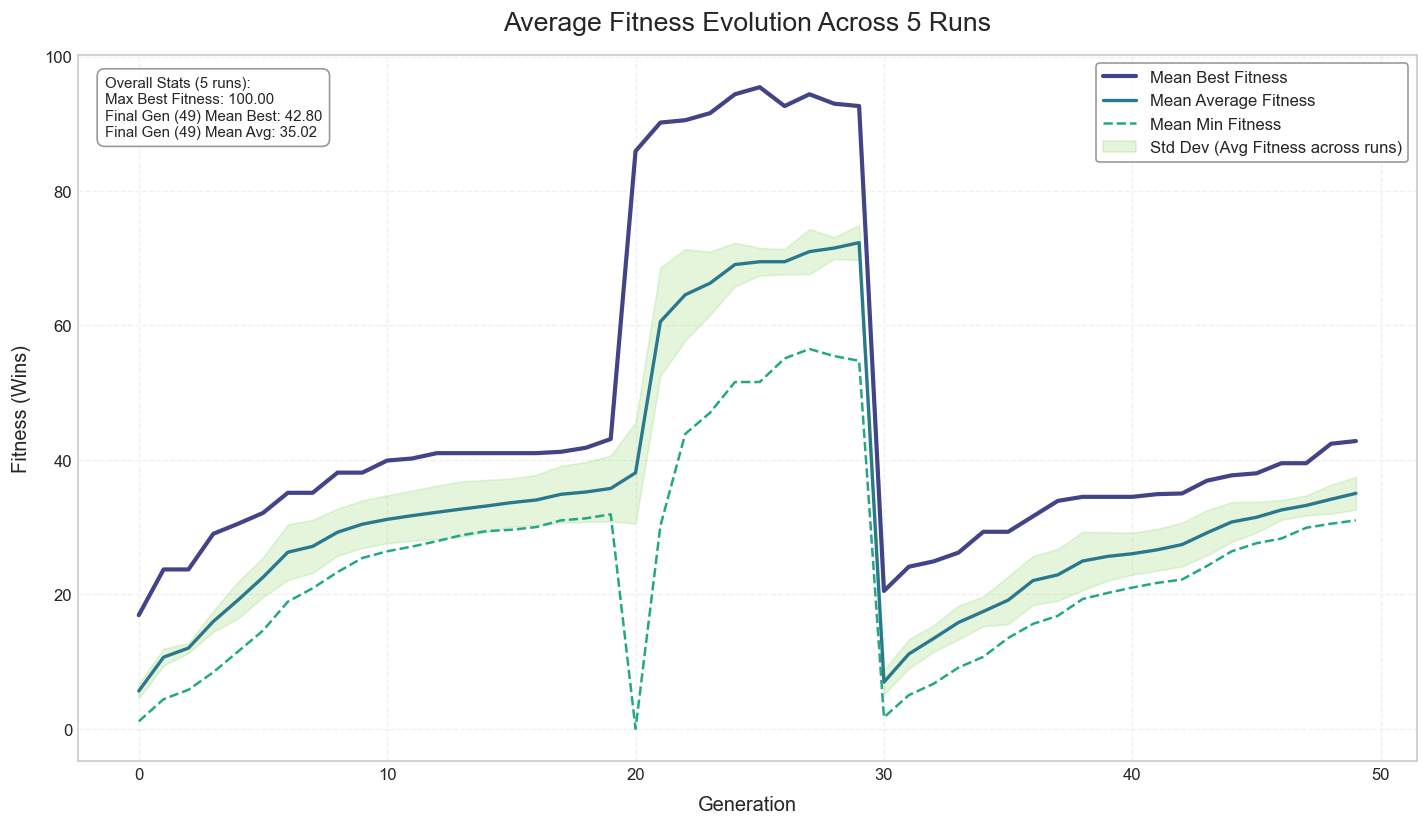
\includegraphics[width=1.0\textwidth]{img/424_fitness_evolution.png}
	\caption{Evolución del fitness sobre las generaciones para la combinación híbrida ganadora.}
	\label{fig:fitness_evolution_424}
\end{figure}

Este comportamiento también se refleja en los pesos de la población a lo largo de las generaciones, como se muestra en la figura \ref{fig:heat_avg_424}. En esta gráfica, en el eje x se muestran las mismas generaciones que en la figura anterior, mientras que en el eje y ahora se muestran los valores medios (a nivel de población) de los 20 pesos de cada bot. Como están normalizados, sus valores van desde 0, con un tono morado, hasta 1, con un tono amarillo. De nuevo, en las generaciones 20 y 30 se observa una especie de reseteo de la población, donde la mayoría de los individuos escogidos serían los hijos de la generación anterior y no sus padres, de ahí que los valores de los pesos parezcan cambiar de forma tan drástica.

Esta gráfica también se puede utilizar para identificar la forma en la que la población le da más o menos prioridad a cada uno de los pesos (tabla de significados en el capítulo \ref{chap:software_bot}). De hecho, fue una de las gráficas más importantes para determinar como se debía ajustar el uso y el cálculo de los pesos en el bot a lo largo del desarrollo de este proyecto. En cierto modo, está mostrando si a la población le ``gusta'' o no usar cada uno de ellos. Por ejemplo, el peso en el que más de acuerdo está la población de que debe ser muy bajo es el de \texttt{C\_TIER\_TAVERN}. Este peso es el que implementa una penalización por dejar cartas disponibles para su compra en la taberna. Cuanto mayor es la calidad de la carta, mayor es la penalización, la cual se va acumulando con cada carta. Tiene sentido que el valor de este peso sea muy bajo, ya que la suma de las penalizaciones de cada carta podría acabar siendo menor que el resto de pesos, desvirtualizando por completo la evaluación del fitness.

Otros valores interesantes pueden ser el de \texttt{POWER\_AMOUNT}, que simplemente le da un valor al cambio de poder entre cada acción. Es un peso extremadamente importante, puesto que el poder sobrante al terminar el turno se convierte en prestigio, la forma más usual de ganar una partida. Por último, destacar el incipiente uso de \texttt{T\_IMPRISONMENT} durante la etapa de coevolución. Parece que la población descubrió el uso de esta carta, pero acabó olvidándolo con el paso a la fase de modo fijo.

\begin{figure}[H]
	\centering
	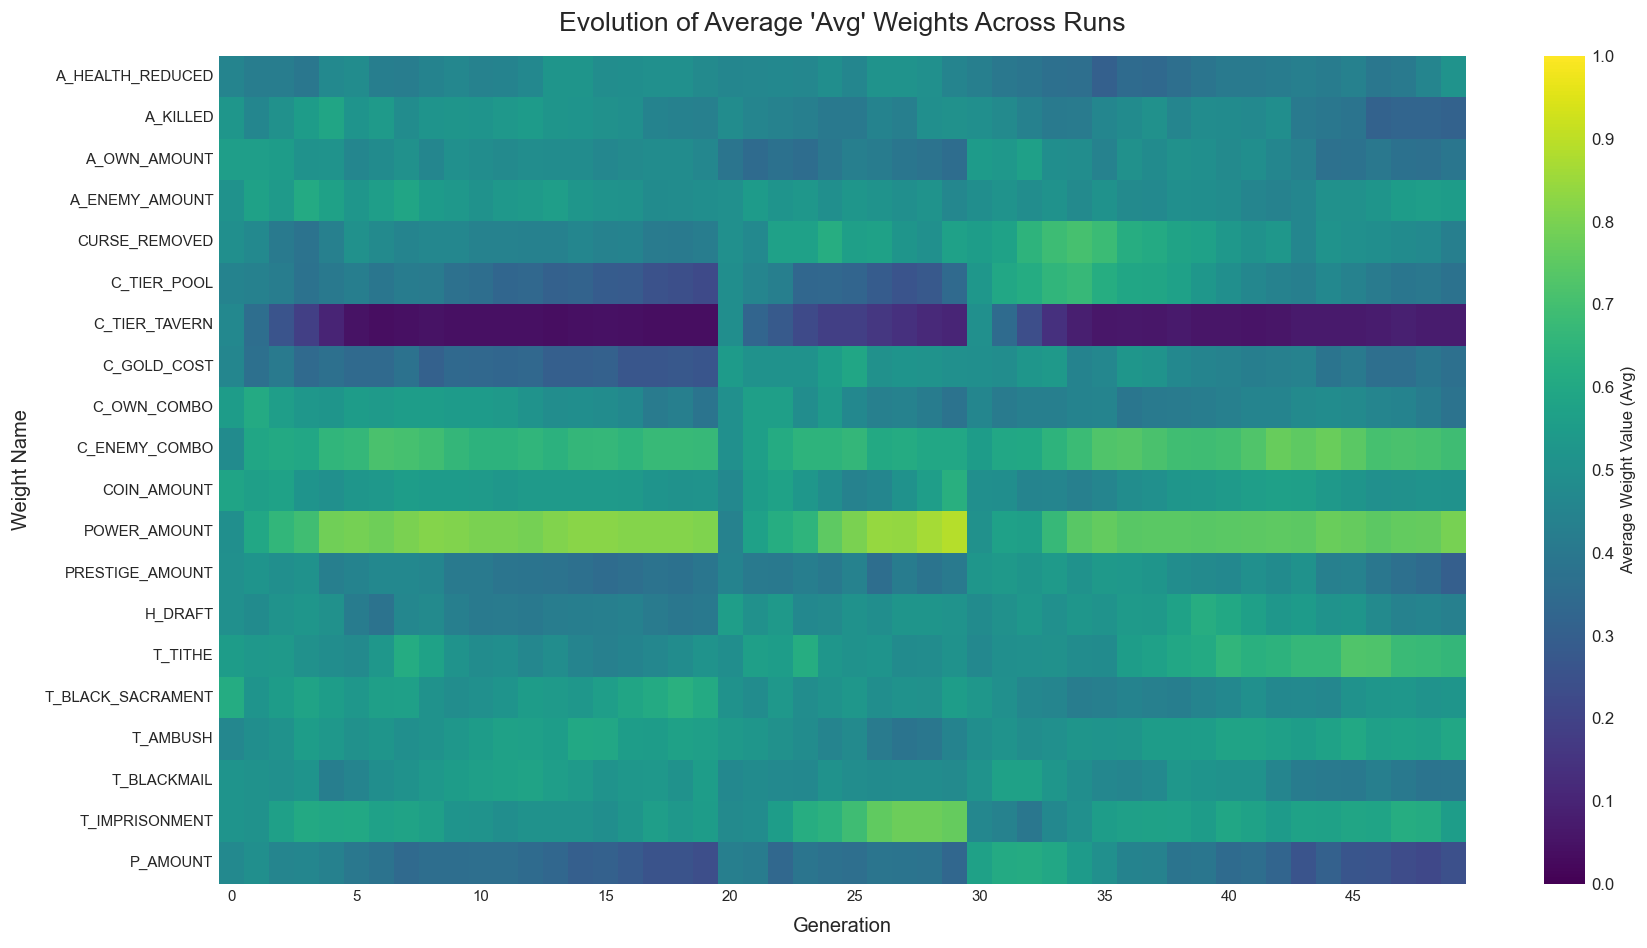
\includegraphics[width=1.0\textwidth]{img/424_heat_avg.png}
	\caption{Evolución de los pesos de la población a lo largo de las generaciones.}
	\label{fig:heat_avg_424}
\end{figure}

En definitiva, el análisis de las configuraciones híbridas revela que no existe una única fórmula para el éxito, pero sí una tendencia clara: las estrategias que logran un balance entre la explotación del conocimiento y la exploración de nuevas tácticas obtienen los mejores resultados. La configuración ganadora, H-3, sugiere que un enfoque que comienza y termina con una fase de entrenamiento guiado, intercalando una fase más corta de competición interna, resulta especialmente efectivo. No obstante, el buen rendimiento de la configuración H-5, dominada por la coevolución, demuestra que también es posible alcanzar un alto rendimiento partiendo de una exploración más abierta. Los resultados de los pesos, visibles en el mapa de calor, refuerzan esta idea, mostrando cómo la población aprende a priorizar ciertas heurísticas, como la importancia del poder o el descarte de cartas de bajo valor, adaptando su estrategia general en función de la naturaleza del desafío al que se enfrenta en cada fase del entrenamiento.

\section{Análisis de los modos de entrenamiento} \label{sec:analisis_modos_entrenamiento}

Tras la ejecución del conjunto experimental que compara los modos de entrenamiento y el salón de la fama (detallada en la Tabla \ref{tab:main_experiments}), se obtuvieron 6 campeones finales, uno por cada configuración evaluada. Para determinar de forma concluyente el rendimiento relativo de cada uno, se llevaron a cabo en este caso dos torneos finales, uno contra bots de referencia y otro entre sí mediante un emparejamiento estilo Round Robin. El primer torneo tuvo exactamente las mismas características que el realizado en la sección anterior, cada bot se enfrentó 5000 veces contra cada uno de los 4 bots de referencia, la mitad como jugador 1 y la otra como jugador 2. La Tabla \ref{tab:resultados_exp_modos} resume el rendimiento de cada campeón, ordenados de mayor a menor según su tasa de victorias global.

\begin{table}[H]
	\centering
	\caption{Rendimiento de los campeones de cada modo de entrenamiento contra oponentes fijos.}
	\label{tab:resultados_exp_modos}
	\small
	\begin{tabular}{@{}lccccccc@{}}
		\toprule
		\textbf{ID} & \textbf{Modo} & \textbf{Tasa Vic.} & \textbf{Tiempo} & \textbf{Patron} & \textbf{Agents} & \textbf{Prestige} & \textbf{Tree}   \\
		\midrule
		B-1         & Fijo F.       & \textbf{50.89\%}   & 2h 53m          & 68.6\%          & \textbf{76.8\%} & 34.1\%            & 24.1\%          \\
		B-5         & Híbrido       & 48.36\%            & 2h 39m          & \textbf{69.8\%} & 65.4\%          & 34.6\%            & 23.7\%          \\
		B-4         & Fijo          & 48.27\%            & \textbf{2h 27m} & 62.0\%          & 63.2\%          & 44.7\%            & 23.3\%          \\
		B-2         & Híbrido  F.   & 41.68\%            & 2h 48m          & 62.9\%          & 57.9\%          & 22.6\%            & 23.2\%          \\
		B-6         & Coevo.        & 35.01\%            & 2h 34m          & 44.0\%          & 21.1\%          & 50.1\%            & \textbf{24.8\%} \\
		B-3         & Coevo. F.     & 32.48\%            & 3h 11m          & 43.7\%          & 17.2\%          & \textbf{52.0\%}   & 17.0\%          \\
		\bottomrule
	\end{tabular}
\end{table}


El campeón del torneo contra los agentes de \textit{Scripts of Tribute} fue el B-1, que logró una tasa de victorias del 50.89\%. Este bot fue entrenado en modo fijo con el salón de la fama activado, lo que significa que los individuos de su población aspiraban constantemente a superar a los campeones de generaciones pasadas. Siguiéndole muy de cerca, los bots B-5 y B-4, que se entrenaron en modo híbrido y fijo respectivamente, lograron tasas de victorias del 48.36\% y 48.27\%. El B-5, es el ganador del torneo de configuraciones híbridas, se puede apreciar que en esta evaluación el porcentaje de victorias solo cambia en un 0.07\% con respecto al anterior, indicando la robustez de la evaluación. Por otro lado, el B-4, que se entrenó en modo fijo sin salón de la fama, demuestra que el modo fijo realmente es el más indicado para este tipo de torneo pues se basa en los mismos pasos que la población de este bot llevó a cabo durante su entrenamiento. Algo curioso es que el salón de la fama en el modo híbrido no solo no aportó un beneficio, sino que incluso pudo haber perjudicado negativamente al rendimiento del bot, ya que el B-2, que también fue entrenado en modo híbrido pero con salón de la fama, obtuvo una tasa de victorias un 7.21\% inferior.

El tiempo de ejecución en este experimento también es bastante similar entre los bots. Ya que también trata de evaluar el impacto del salón de la fama, se intentó que el tiempo de entrenamiento de las 3 configuraciones que lo usaban tuvieran un tiempo similar entre sí. En este caso, las configuraciones marcadas con una ``F'' al final de su nombre son las que usan el salón de la fama, y van desde 2h y 48 minutos hasta 3 horas y 11 minutos. Esto supone una diferencia de tiempo del 13.7\%, lo que demuestra que el coste computacional entre los 3 modos de entrenamiento, cuando tienen el salón de la fama activado, es similar.

Al ver como evoluciona el fitness de la configuración ganadora B-1 en la figura \ref{fig:fixed_fitness_evolution}, se puede observar que la evolución del fitness es bastante estable a lo largo de las 50 generaciones. La tasa de victorias sube rápidamente durante las primeras generaciones y la mejora se ralentiza a partir de la generación 25. Aun así, justo al final del entrenamiento se produce una ligera subida, lo que indica que el bot podría haber seguido mejorando si se hubiera continuado entrenando. Este es el comportamiento típico de un algoritmo evolutivo, donde la población se adapta a un entorno cambiante y mejora su rendimiento a lo largo del tiempo hasta llegar a un punto de saturación. Un punto a destacar es como durante la mayor subida de rendimiento, la desviación típica del fitness de cada una de las 5 carreras sube mucho, indicando altas diferencias entre ellas. Sin embargo, conforme va avanzando el entrenamiento la desviación baja, lo que indica que en los 5 casos el rendimiento de la población se va homogeneizando.

\begin{figure}[H]
	\centering
	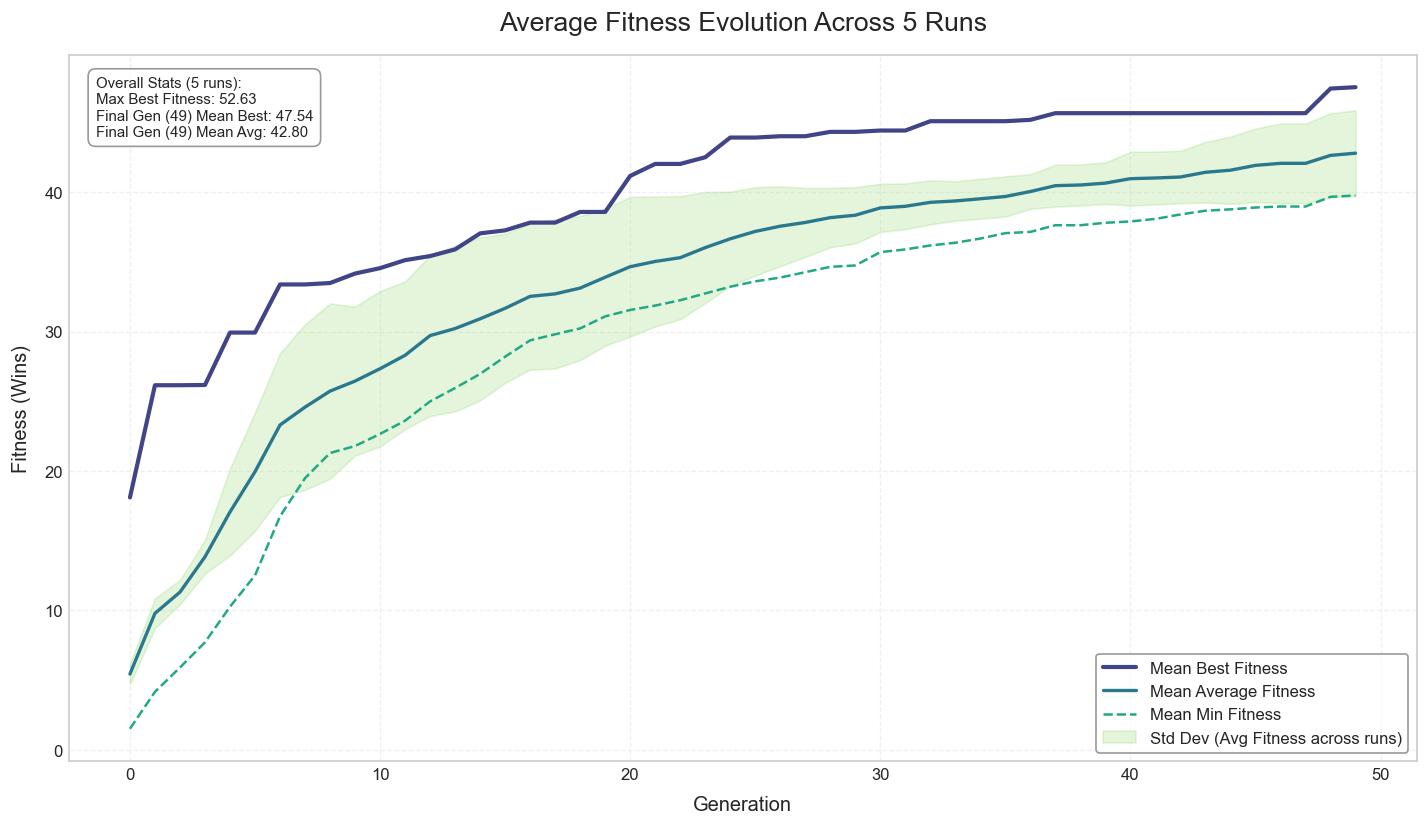
\includegraphics[width=1.0\textwidth]{img/fixed_fitness_evolution.png}
	\caption{Evolución del fitness sobre las generaciones para la combinación fija ganadora.}
	\label{fig:fixed_fitness_evolution}
\end{figure}

Al centrarnos en los pesos de los mejores individuos de la configuración ganadora, se puede generar un mapa de calor parecido al de la figura \ref{fig:heat_avg_424} de la sección anterior. En la figura \ref{fig:fixed_heat_best} se ve este caso específico, el cual únicamente muestra como cambian los pesos de la élite. La primera diferencia aparente se ve en como de los pesos cambian de forma más drástica a lo largo de las generaciones. En la figura \ref{fig:heat_avg_424}, los valores de los pesos se mantienen bastante estables de generación en generación, mientras que en este caso se pueden encontrar saltos de hasta un 30\% en un solo paso. En ambos la evolución de \textit{C\_TIER\_TAVERN} se ha desarrollado hasta valores muy bajos, pero en este caso el valor de \textit{C\_TIER\_POOL} es mucho más pequeño también, llegado a ser prácticamente 0. Este peso se utiliza para comparar el valor de las cartas de la mano del EvolutionaryBot con las de su rival, y parece que la población ha aprendido que no es necesario tener mucho en cuenta este valor. Una razón de este comportamiento puede ser que el bot no tiene memoria, por lo que no puede planificar a largo plazo, y por tanto no le interesa tanto el valor de las cartas que tiene en un cierto momento en la mano. Por último, destacar que esta población también parece haber descubierto el uso de la carta \textit{Imprisonment}, ya que el valor de su peso es bastante alto, lo que indica que tanto en el modo fijo como en el coevolutivo, la población puede aprender a usar esta carta de forma efectiva.

\begin{figure}[H]
	\centering
	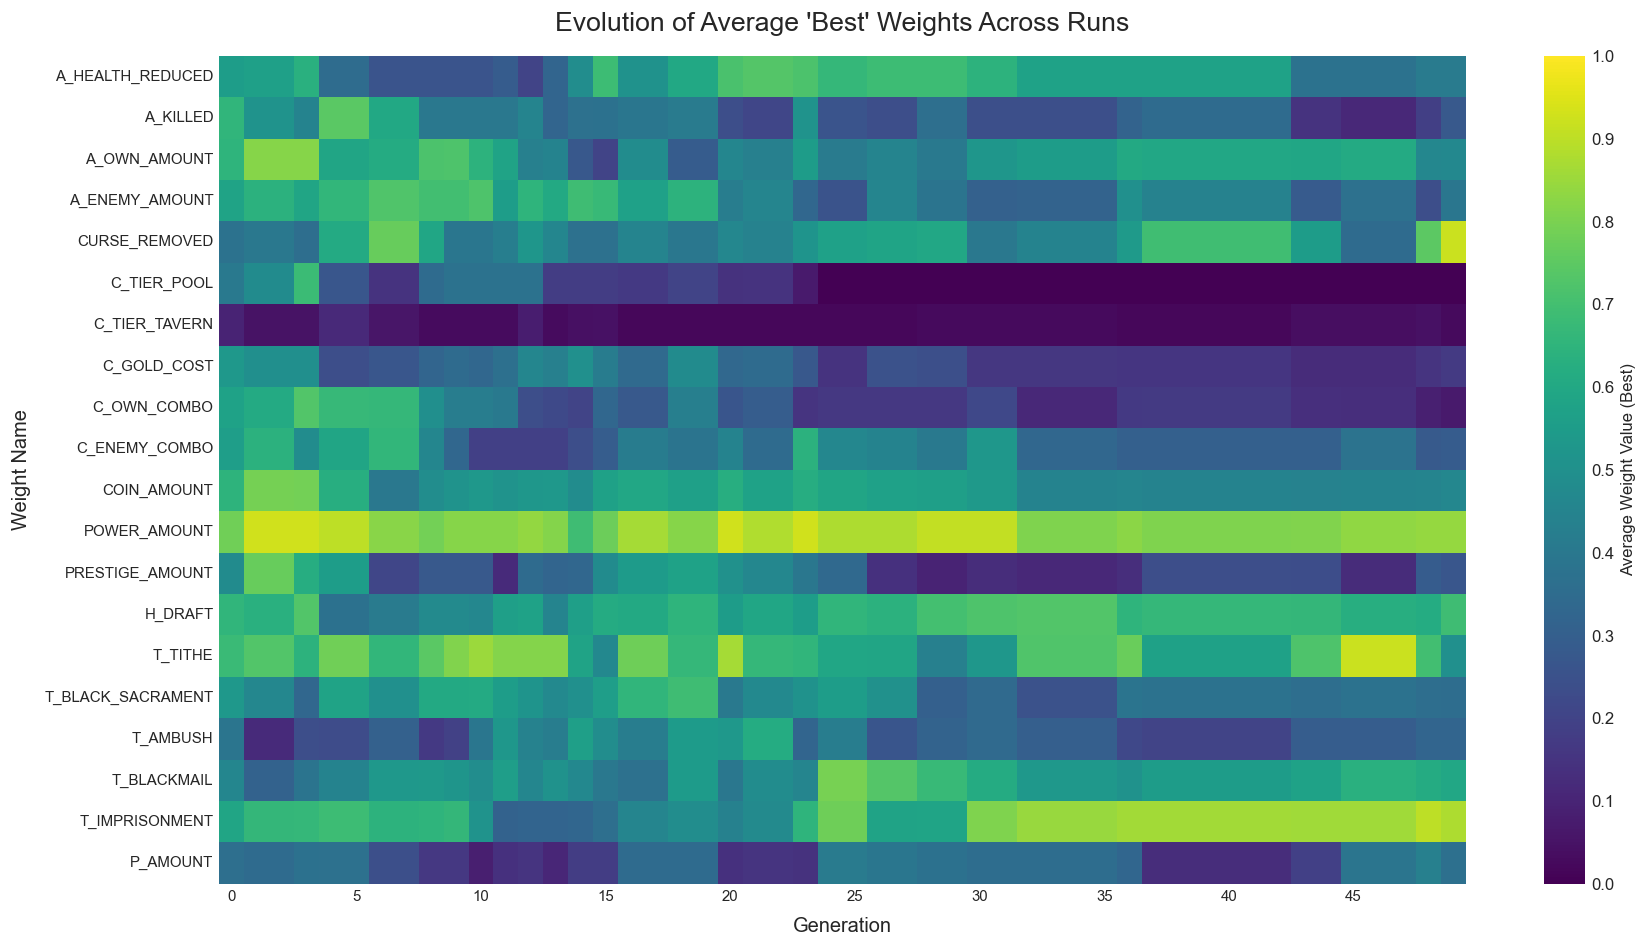
\includegraphics[width=1.0\textwidth]{img/fixed_heat_best.png}
	\caption{Evolución de los pesos del mejor individuo de la combinación fija ganadora a lo largo de las generaciones.}
	\label{fig:fixed_heat_best}
\end{figure}

Para ver los pesos de forma más precisa, se creó la figura \ref{fig:fixed_fitness_evolution}, donde se muestran los del mejor individuo de la configuración B-1 en su última generación. Este probablemente haya sido el individuo que originó ese ligero aumento del fitness al final del entrenamiento. Aquí se puede ver que el valor de \textit{C\_TIER\_POOL} es 0, lo que indica que el bot ha descartado por completo el uso de este peso, al contrario que con \textit{C\_TIER\_TAVERN}, que tiene un valor de 0.025. El peso con mayor valor es \textit{CURSE\_REMOVED}, que da un valor positivo se el bot se quita una maldición y uno negativo si se la quita al oponente. Este peso es muy importante, ya que las maldiciones son una de las formas más efectivas de entorpecer el turno de un jugador, y por tanto, su eliminación puede ser crucial para ganar una partida.

\begin{figure}[H]
	\centering
	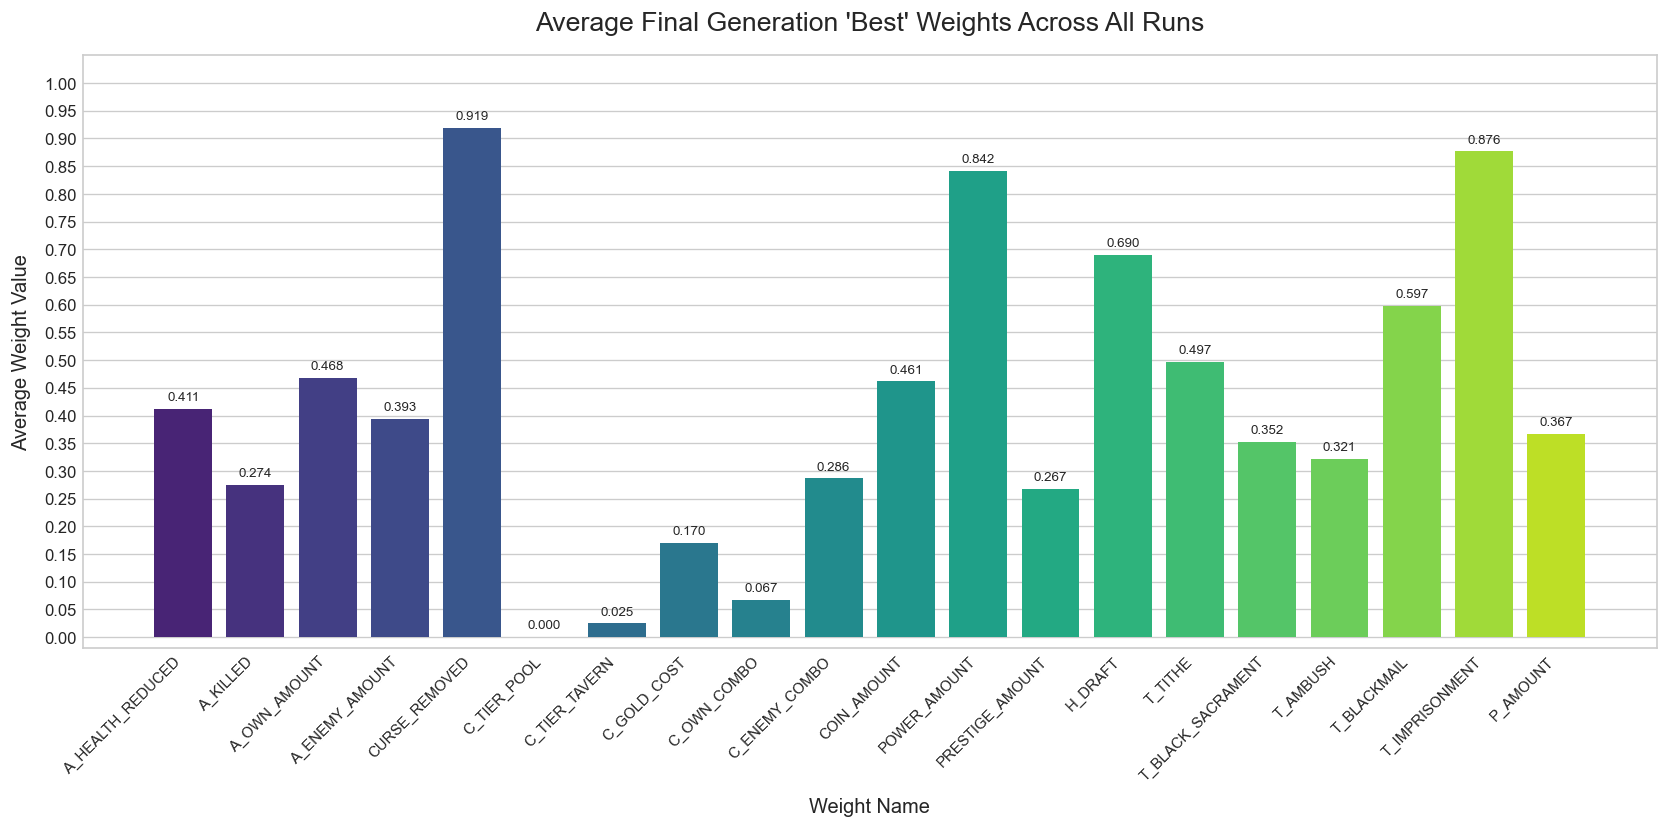
\includegraphics[width=1.0\textwidth]{img/fixed_avg_weights_best.png}
	\caption{Valores finales de los pesos del mejor individuo de la combinación fija ganadora.}
	\label{fig:fixed_avg_weights_best}
\end{figure}

Volviendo a los resultados de la tabla \ref{tab:resultados_exp_modos}, un último aspecto a destacar es la clara diferencia entre los porcentajes de victorias de los modos fijos e híbridos frente a los de coevolución. Donde los primeros logran tasas buenas, como contra el \textit{MaxAgentsBot}, en los bots coevolutivos son nefastas, mientras que estos resultados se invierten contra el \textit{MaxPrestigeBot}. Curiosamente, esto no ocurre contra el \textit{DecisionTreeBot}, donde los bots fijos e híbridos logran tasas de victoria similares, y el coevolutivo sin salón de la fama logra la tasa más alta, pero el que no utiliza este sistema obtiene la peor tasa de victorias. Quizás este comportamiento indica que el salón de la fama en modo coevolutivo produce una sobreespecialización en el bot para luchar contra si mismo, y cuando se enfrenta a bots fijos, su rendimiento puede llegar a ser incluso peor que el de un bot que no ha sido entrenado con este sistema.

Para entender mejor el nivel de especialización de los bots, se realizó un segundo benchmark en el que los 6 campeones se enfrentaron entre sí en un torneo de todos contra todos, jugando otras 5000 partidas en cada emparejamiento. La tabla \ref{tab:coevo_benchmark_resultados} presenta la matriz de resultados de este torneo, mostrando la tasa de victorias de cada campeón contra cada oponente. Adicionalmente, la tabla \ref{tab:coevo_ranking_final} ofrece un resumen final, ordenando a los campeones según su rendimiento en las 25000 partidas totales del torneo.

\begin{table}[H]
	\centering
	\caption{Matriz de resultados del torneo EvolutionaryBot vs EvolutionaryBot.}
	\label{tab:coevo_benchmark_resultados}
	\begin{tabular}{@{}lcccccc@{}}
		\toprule
		\textbf{vs}  & \textbf{B-1} & \textbf{B-2} & \textbf{B-3} & \textbf{B-4} & \textbf{B-5} & \textbf{B-6} \\
		\midrule
		\textbf{B-1} & ---          & 41.5\%       & 22.0\%       & 40.4\%       & 47.5\%       & 23.4\%       \\
		\textbf{B-2} & 58.5\%       & ---          & 3.4\%        & 44.6\%       & 51.3\%       & 4.3\%        \\
		\textbf{B-3} & 78.0\%       & 96.6\%       & ---          & 99.3\%       & 77.2\%       & 61.1\%       \\
		\textbf{B-4} & 59.6\%       & 55.4\%       & 0.7\%        & ---          & 50.8\%       & 3.4\%        \\
		\textbf{B-5} & 52.5\%       & 48.7\%       & 22.8\%       & 49.2\%       & ---          & 26.6\%       \\
		\textbf{B-6} & 76.6\%       & 95.7\%       & 38.9\%       & 96.6\%       & 73.4\%       & ---          \\
		\bottomrule
	\end{tabular}
\end{table}

\begin{table}[H]
	\centering
	\caption{Clasificación final del torneo EvolutionaryBot vs EvolutionaryBot.}
	\label{tab:coevo_ranking_final}
	\begin{tabular}{@{}lccc@{}}
		\toprule
		\textbf{ID} & \textbf{Modo} & \textbf{Tasa Vic.} & \textbf{Vic. Totales} \\
		\midrule
		B-3         & Coevo. F.     & 82.43\%            & (20607 / 25000)       \\
		B-6         & Coevo.        & 76.25\%            & (19063 / 25000)       \\
		B-5         & Híbrido       & 39.97\%            & (9992 / 25000)        \\
		B-1         & Fijo F.       & 34.95\%            & (8738 / 25000)        \\
		B-4         & Fijo          & 33.98\%            & (8494 / 25000)        \\
		B-2         & Híbrido F.    & 32.42\%            & (8106 / 25000)        \\
		\bottomrule
	\end{tabular}
\end{table}

De la misma forma que el ganador del torneo contra los bots de referencia se entrenó en modo fijo con salón de la fama, el campeón del torneo entre los EvolutionaryBots fue el B-3, que se entrenó en modo coevolutivo con salón de la fama. Este conjunto de pesos logró una tasa de victorias del 82.43\% contra los demás, acabando muy por encima de los bots entrenados en modo fijo o híbrido. El segundo puesto fue para el B-6, que se entrenó en modo coevolutivo sin salón de la fama. Se deduce, por tanto, que el tipo de oponente contra el que se entrena el bot tiene un impacto muy significativo en su rendimiento final. Los agentes entrenados específicamente para luchar contra otros EvolutionaryBots son especialmente buenos en este tipo de enfrentamientos, mientras que los entrenados contra los bots de referencia tienen un rendimiento mucho mejor únicamente contra ellos. El caso más radical es el del B-3 vs B-4, el cual logró una tasa de victorias del 99.3\% favorable al B-3.

Al analizar la evolución del fitness del campeón coevolutivo B-3 \ref{fig:coevo_fitness_evolution}, se observa un tercer comportamiento muy característico. A diferencia de los entrenamientos en modo fijo, el fitness del mejor individuo no muestra una subida constante, sino que tiende a disminuir ligeramente a lo largo de las generaciones. Este fenómeno, lejos de ser una anomalía, es una manifestación del clásico ``Efecto Reina Roja'' en sistemas evolutivos. Este efecto describe cómo en un entorno competitivo, los individuos deben mejorar constantemente solo para mantener su posición relativa frente a una población de adversarios que también está evolucionando \cite{wikipedia_red_2025}. Esto explica perfectamente los resultados observados. Aunque el campeón de la generación 40 es, con toda seguridad, un agente mucho más fuerte que el de la generación 10, su tasa de victorias se mide contra oponentes cada vez más duros. La mejora constante del conjunto de la población provoca que el dominio del campeón no aumente e incluso se reduzca, a pesar de la clara ventaja que sigue manteniendo sobre los demás individuos de su propia generación.

\begin{figure}[H]
	\centering
	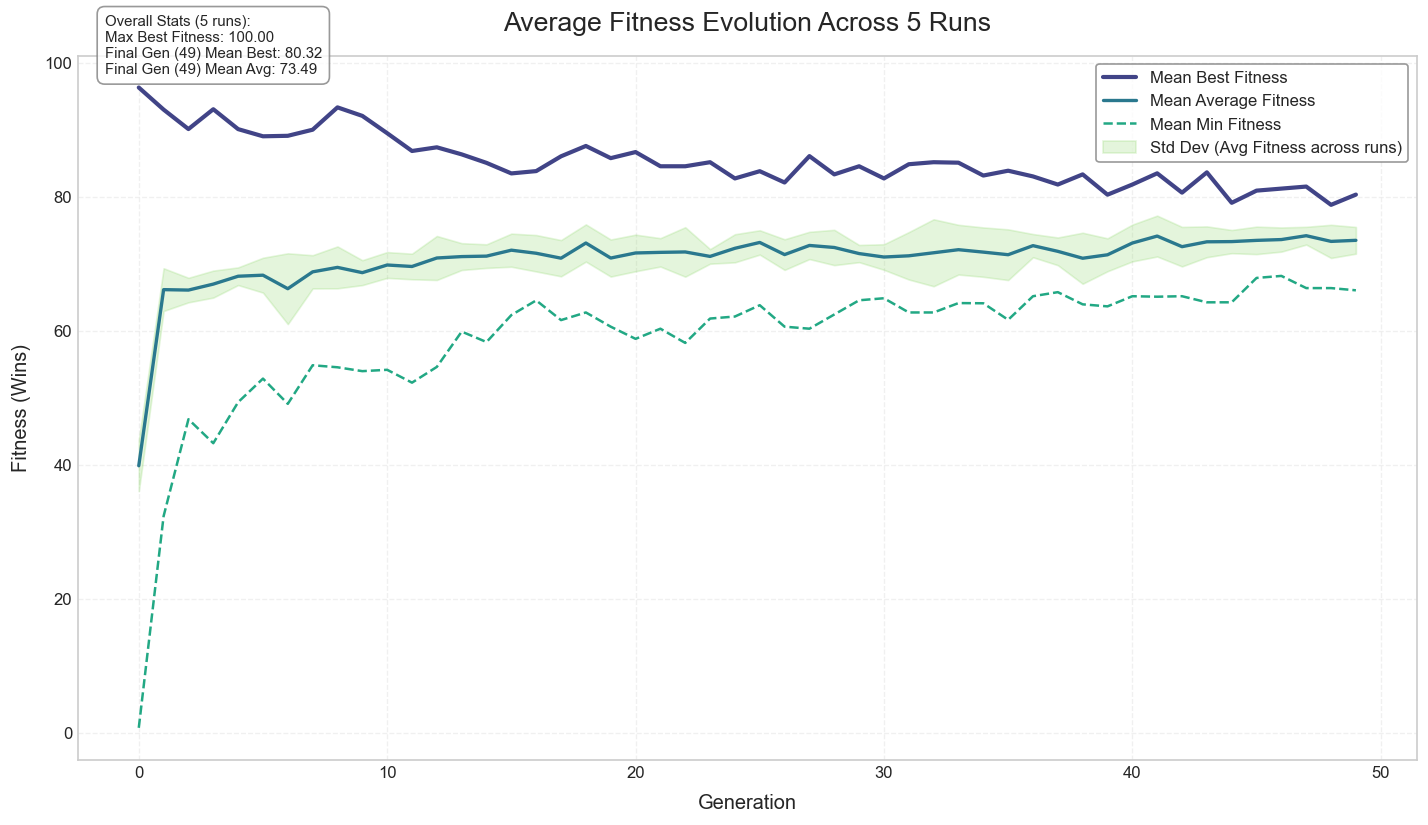
\includegraphics[width=1.0\textwidth]{img/coevo_fitness_evolution.png}
	\caption{Evolución del fitness del campeón del torneo EvolutionaryBot vs EvolutionaryBot.}
	\label{fig:coevo_fitness_evolution}
\end{figure}

El último tipo de gráfico que se generó para este trabajo es un Box plot de los pesos de la última generación. En este caso, cada valor de la figura \ref{fig:coevo_final_weights_avg} representa la media de los pesos de toda la población en cada una de las 5 carreras de la configuración coevolutiva con salón de la fama (de donde salió B-3). Se puede ver como hay tanto pesos en los que las poblaciones de las 5 carreras están de acuerdo, como en los que hay una gran discrepancia entre ellos. Por ejemplo, \textit{C\_TIER\_POOL} y \textit{POWER\_AMOUNT} tiene una discrepancia menor a 0.05 entre las 5 poblaciones, en el caso del primer peso para un valor cercano a 0 y en el segundo para uno cercano a 1. También se encuentran pesos con una distribución de valores muy grande, como \textit{C\_GOLD\_COST}, el cual trata de medir la importancia del coste en oro de las cartas. En ese caso, las poblaciones no se pusieron de acuerdo, ya que sus valores van desde 0.1 hasta 0.85. Este tipo de discrepancias son normales en los algoritmos evolutivos, ya que cada individuo ha evolucionado de forma independiente y ha encontrado su propia forma de jugar al juego. Ahora bien, es posible que con las suficientes generaciones, las poblaciones acabasen convergiendo hacia un conjunto de pesos más homogéneo, pero el tiempo de entrenamiento no fue suficiente para llegar a ese punto.

Se intentaron realizar experimentos con un mayor número de generaciones, pero debido a problemas técnicos con el servidor de entrenamiento, no fue posible. Con todo, los resultados obtenidos se consideran lo suficientemente representativos como para cumplir los objetivos del proyecto.

\begin{figure}[H]
	\centering
	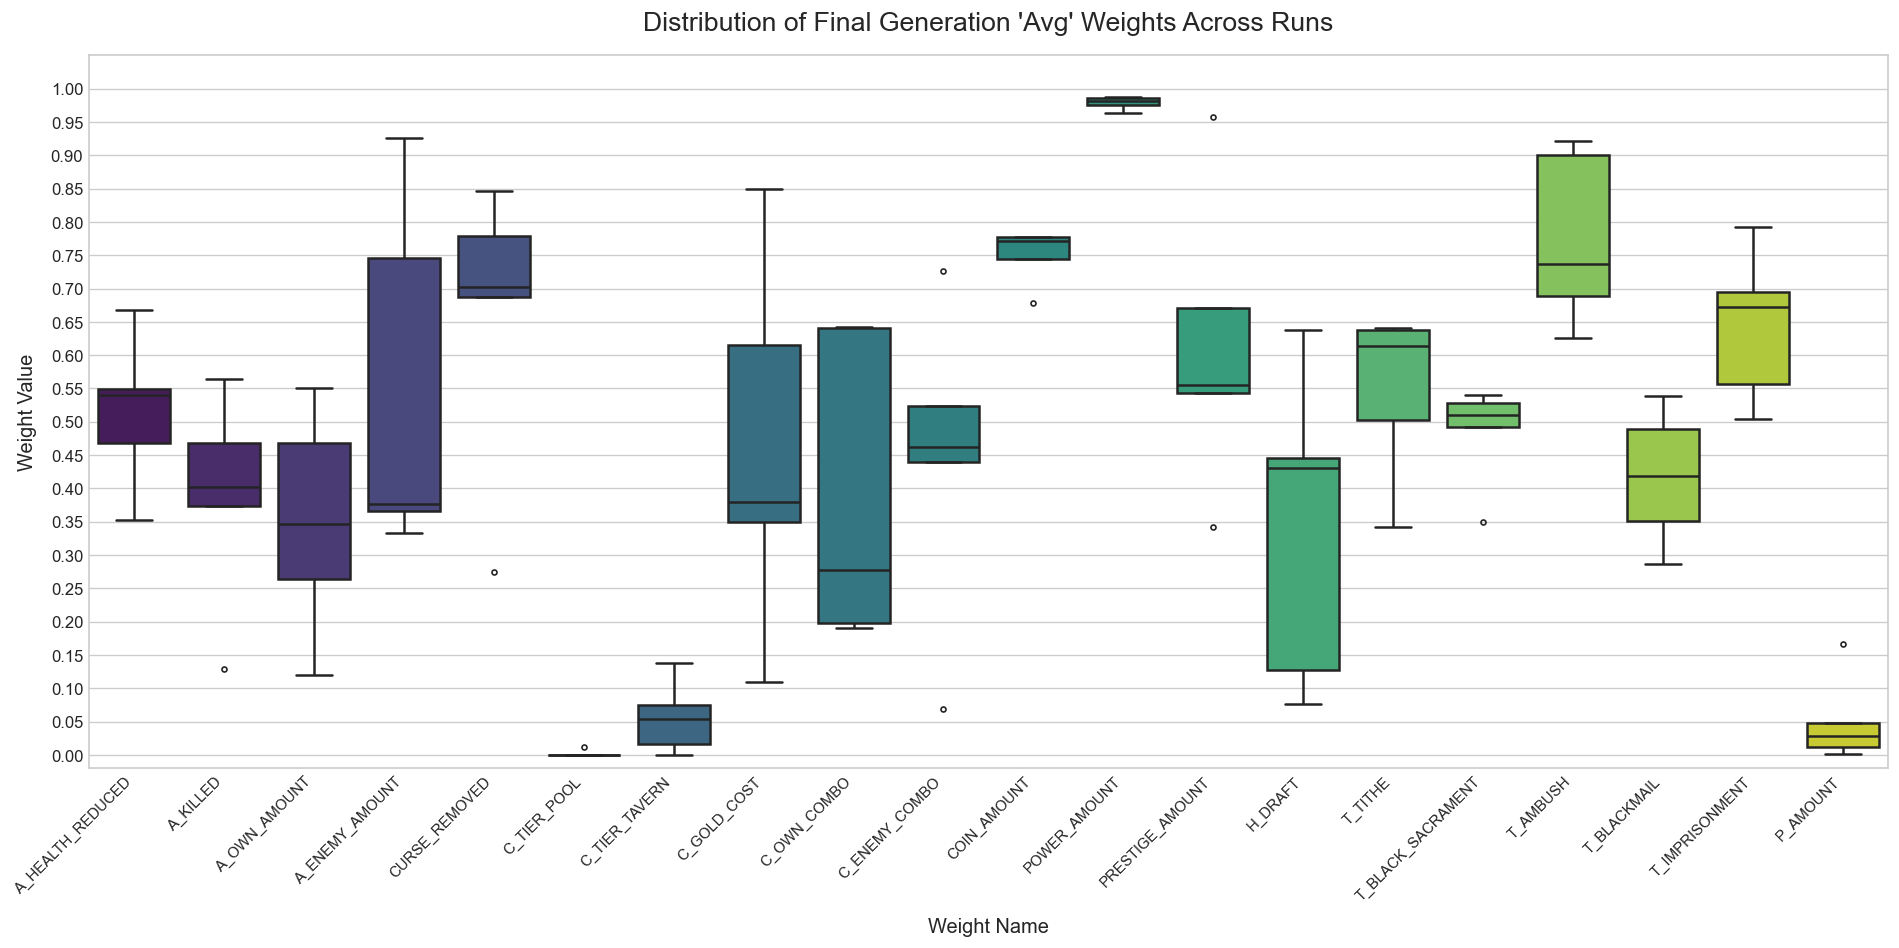
\includegraphics[width=1.0\textwidth]{img/coevo_final_weights_avg.png}
	\caption{Distribución de los pesos de la población final del agente coevolutivo.}
	\label{fig:coevo_final_weights_avg}
\end{figure}

\section{Análisis del salón de la fama} \label{sec:analisis_salon_fama}

El impacto del salón de la fama interno es uno de los resultados más reveladores de la fase experimental, ya que su efectividad demuestra estar intrínsecamente ligada a la estabilidad y al tipo del entorno de entrenamiento. Lejos de ser una mejora universal, su beneficio depende directamente de la consistencia del objetivo que el algoritmo evolutivo intenta optimizar en cada momento.

Los resultados son claros y contundentes cuando se analiza el rendimiento en los modos de entrenamiento enfocados. Tanto en el modo fijo como en el coevolutivo, la presencia del salón de la fama produjo a los campeones con mejores resultados. El agente B-1 (entrenado en modo fijo con salón de la fama) fue el ganador absoluto en el benchmark contra oponentes estáticos. De forma análoga, el agente B-3 (entrenado en modo coevolutivo con salón de la fama) dominó de manera aplastante el torneo de todos contra todos. Esto confirma la hipótesis inicial: en un entorno de entrenamiento consistente, el salón de la fama actúa como un mecanismo de memoria crucial.

Sin embargo, el resultado más sorprendente se observó en el modo híbrido. El agente B-2, entrenado con una planificación híbrida y con el salón de la fama activado, obtuvo un rendimiento significativamente inferior (una tasa de victorias del 41.68\%) que su contraparte B-5 (48.36\%), entrenada con la misma planificación pero sin el salón de la fama. Este fenómeno, aparentemente contraintuitivo, puede explicarse por la propia naturaleza cambiante del modo híbrido. Al cambiar el modo de evaluación de un segmento a otro (por ejemplo, de fijo a coevolución), el ``objetivo'' que la población debe optimizar también cambia. Un campeón que era excelente en el segmento de modo fijo podría ser añadido al salón de la fama, para luego convertirse en un oponente poco representativo o incluso contraproducente durante el siguiente segmento de coevolución. Al mantener a estos campeones ``desactualizados'' en la memoria, el salón de la fama podría estar entorpeciendo el proceso de adaptación de la población al nuevo entorno, ``confundiendo'' el cálculo del \textit{fitness} y perjudicando el resultado final.

Por lo tanto, se puede concluir que el salón de la fama es una herramienta de gran utilidad, pero su implementación debe adaptarse al objetivo de la población. Resulta ser un componente muy beneficioso en entornos de entrenamiento estables y homogéneos, pero puede llegar a ser perjudicial en escenarios dinámicos donde el objetivo de la optimización cambia a lo largo de la propia carrera evolutiva.

Con la finalización de esta fase experimental, se han cumplido los objetivos \textbf{OG5} y \textbf{OG6} del proyecto. Se ha evaluado cuantitativamente el rendimiento del agente entrenado mediante diferentes estrategias, utilizando métricas relevantes como la tasa de victorias y el tiempo de entrenamiento. Además, se ha realizado un análisis comparativo de la efectividad y eficiencia de las estrategias de optimización implementadas, discutiendo sus ventajas y desventajas. Así, se concluye el cumplimiento de todos los objetivos específicos del proyecto.